\section{Structure from Motion và Visual SLAM: Xây dựng Bản đồ từ Ảnh}
\label{sec:sfm_slam}

\subsection{Giới thiệu: Từ Hình học đến Bản đồ}
\label{subsec:sfm_intro}

Trong các phần trước của chương này, chúng ta đã xây dựng một bộ công cụ hình học ấn tượng: mô hình pinhole, ma trận nội tại $K$, các tham số ngoại tại $(R, t)$, hình học epipolar, và tam giác hóa. Tất cả những công cụ này đã được giới thiệu như những công trình toán học thuần túy.

Nhưng một câu hỏi tự nhiên xuất hiện: \textit{Những công cụ này thực sự giải quyết được bài toán gì trong thực tế?}

Câu trả lời là hai bài toán quan trọng bậc nhất trong thị giác 3D: \textbf{Structure from Motion (SfM)} và \textbf{Visual SLAM}.

\begin{mdframed}[style=infobox]
    \textbf{Bài toán Ngược của Camera}

    Nếu chương này bắt đầu bằng bài toán \textit{xuôi} (forward problem): biết vị trí camera và điểm 3D, hãy tính ảnh 2D — thì SfM và SLAM giải bài toán \textit{ngược} (inverse problem): biết nhiều ảnh 2D, hãy khôi phục vị trí camera \textit{và} cấu trúc 3D của cảnh.
\end{mdframed}

\subsection{Structure from Motion (SfM)}
\label{subsec:sfm}

\subsubsection{Bài toán: Tái dựng 3D từ Tập ảnh Tùy ý}
\label{subsubsec:sfm_problem}

SfM giải bài toán sau: cho một tập hợp $N$ ảnh của cùng một cảnh tĩnh, được chụp từ các góc độ tùy ý (không cần biết trước thứ tự hay vị trí camera), hãy đồng thời phục hồi:
\begin{itemize}
    \item \textbf{Tư thế (pose) của từng camera}: ma trận $[R_i | t_i]$ cho mỗi ảnh $i$.
    \item \textbf{Tọa độ 3D} của các điểm đặc trưng quan sát được trong nhiều ảnh.
\end{itemize}

\subsubsection{Pipeline SfM Incremental}
\label{subsubsec:sfm_pipeline}

Pipeline SfM tiêu chuẩn (theo kiểu incremental, như COLMAP \cite{Schonberger2016}) hoạt động theo các bước sau:

\begin{enumerate}
    \item \textbf{Phát hiện và So khớp Đặc trưng:} Phát hiện keypoints (SIFT, SuperPoint...) trong mỗi ảnh. Tìm các điểm tương ứng (correspondences) giữa mọi cặp ảnh.

    \item \textbf{Ước tính Hình học Hai ảnh:} Với mỗi cặp ảnh có đủ correspondences, ước tính ma trận cơ bản $F$ (hoặc ma trận thiết yếu $E$) bằng RANSAC. Phân rã $E$ để tính $[R|t]$ tương đối.

    \item \textbf{Khởi tạo với Cặp ảnh Đầu tiên:} Chọn cặp ảnh có nhiều correspondences nhất làm điểm khởi đầu. Tam giác hóa để có tập điểm 3D ban đầu.

    \item \textbf{Đăng ký ảnh mới (Incremental Registration):} Lần lượt thêm từng ảnh mới bằng cách:
    \begin{itemize}
        \item Tìm correspondences giữa ảnh mới và các điểm 3D đã biết.
        \item Giải bài toán \textbf{Perspective-n-Point (PnP)} để tính pose của camera mới.
        \item Tam giác hóa thêm các điểm 3D mới.
    \end{itemize}

    \item \textbf{Bundle Adjustment:} Tối ưu hóa \textit{đồng thời} toàn bộ poses của camera và tọa độ 3D để cực tiểu hóa tổng sai số tái chiếu (reprojection error):
    \[
        \min_{\{R_i, t_i\}, \{X_j\}} \sum_{i,j} \left\| \pi(K_i [R_i | t_i] X_j) - x_{ij} \right\|^2
    \]
    trong đó $\pi$ là phép chiếu phối cảnh và $x_{ij}$ là vị trí quan sát được của điểm $j$ trong ảnh $i$.
\end{enumerate}

\begin{center}
    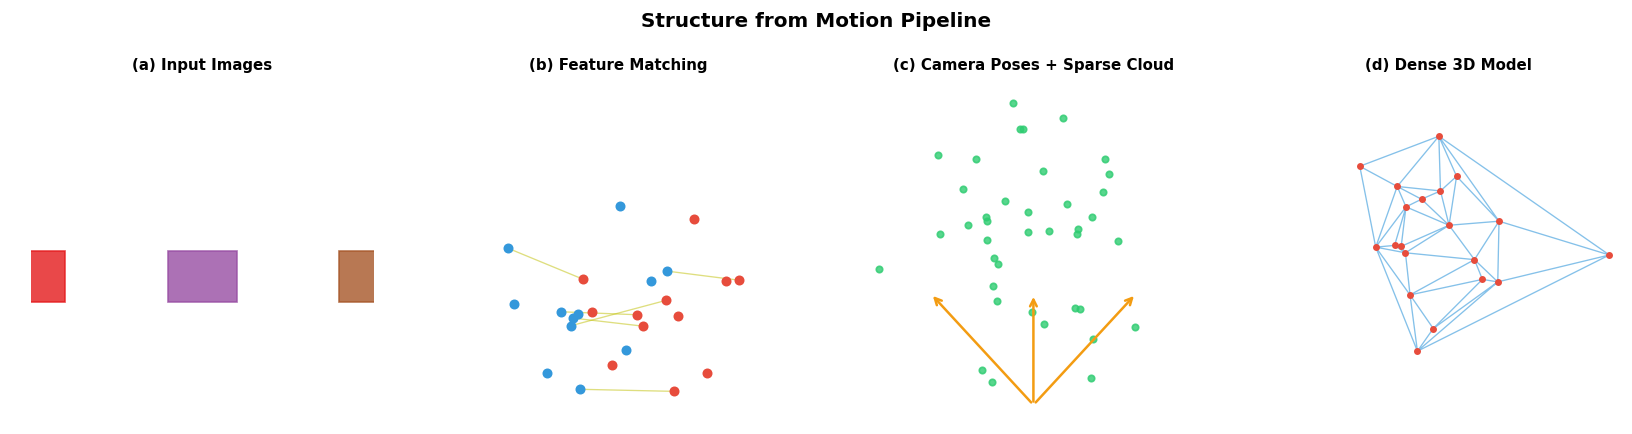
\includegraphics[width=0.9\textwidth]{images/sfm_pipeline.png}
    \captionof{figure}{Pipeline SfM từ tập ảnh tùy ý đến đám mây điểm 3D. (a) Ảnh đầu vào từ nhiều góc độ. (b) So khớp đặc trưng. (c) Poses camera và đám mây điểm thưa (sparse point cloud). (d) Sau dense reconstruction, thu được mô hình 3D dày đặc.}
    \label{fig:sfm_pipeline}
\end{center}

\subsubsection{COLMAP: Công cụ SfM Thực tế}
\label{subsubsec:colmap}

COLMAP \cite{Schonberger2016} là phần mềm SfM mã nguồn mở tiêu chuẩn trong cộng đồng CV. Nó được sử dụng rộng rãi để tạo dữ liệu 3D cho:
\begin{itemize}
    \item Huấn luyện NeRF và Gaussian Splatting (sẽ học ở Chương 8).
    \item Xây dựng bản đồ 3D cho AR/VR.
    \item Tái dựng di tích lịch sử từ hình ảnh.
\end{itemize}

Cùng với SfM, pipeline hoàn chỉnh thường bao gồm bước \textbf{Multi-View Stereo (MVS)} để tái dựng bề mặt dày đặc (dense mesh) từ đám mây điểm thưa.

\subsection{Visual SLAM: Đồng thời Định vị và Lập bản đồ}
\label{subsec:visual_slam}

\subsubsection{Bài toán: Robot không biết mình đang ở đâu}
\label{subsubsec:slam_problem}

SfM hoạt động theo kiểu \textit{offline}: thu thập toàn bộ ảnh trước, xử lý sau. Nhưng một robot di chuyển trong không gian không thể chờ đến khi thu thập xong—nó cần \textit{biết vị trí của mình ngay lập tức} để ra quyết định.

\textbf{Visual SLAM} (Simultaneous Localization and Mapping) giải quyết bài toán này trong thời gian thực:
\begin{quote}
    \textit{Một robot không biết gì về môi trường xung quanh. Chỉ với camera, nó phải đồng thời xây dựng bản đồ (map) của môi trường VÀ xác định vị trí của mình (localize) trong bản đồ đó — và hai nhiệm vụ này phụ thuộc lẫn nhau.}
\end{quote}

Đây là một bài toán gà-trứng kinh điển: để định vị cần có bản đồ; để xây bản đồ cần biết vị trí.

\subsubsection{Kiến trúc của một Hệ thống Visual SLAM}
\label{subsubsec:slam_architecture}

Một hệ thống Visual SLAM điển hình (như ORB-SLAM3 \cite{Campos2021}) gồm các module:

\begin{enumerate}
    \item \textbf{Tracking (Theo dõi):} Ước tính pose của camera tại mỗi khung hình mới bằng cách so khớp đặc trưng với keyframes gần đây. Module này chạy với tần suất cao (theo frame rate của camera).

    \item \textbf{Local Mapping (Lập bản đồ cục bộ):} Chèn keyframes mới vào bản đồ, tam giác hóa thêm điểm 3D, và chạy Local Bundle Adjustment để tinh chỉnh khu vực lân cận.

    \item \textbf{Loop Closing (Phát hiện vòng lặp):} Nhận ra khi robot quay trở lại nơi đã từng đi qua, và "đóng vòng lặp" để loại bỏ sai số tích lũy (drift). Đây là bước phân biệt SLAM với odometry đơn thuần.

    \item \textbf{Global Optimization:} Sau khi phát hiện loop, chạy tối ưu hóa toàn cục (Pose Graph Optimization) để phân bổ sai số đều trên toàn bộ trajectory.
\end{enumerate}

\begin{center}
    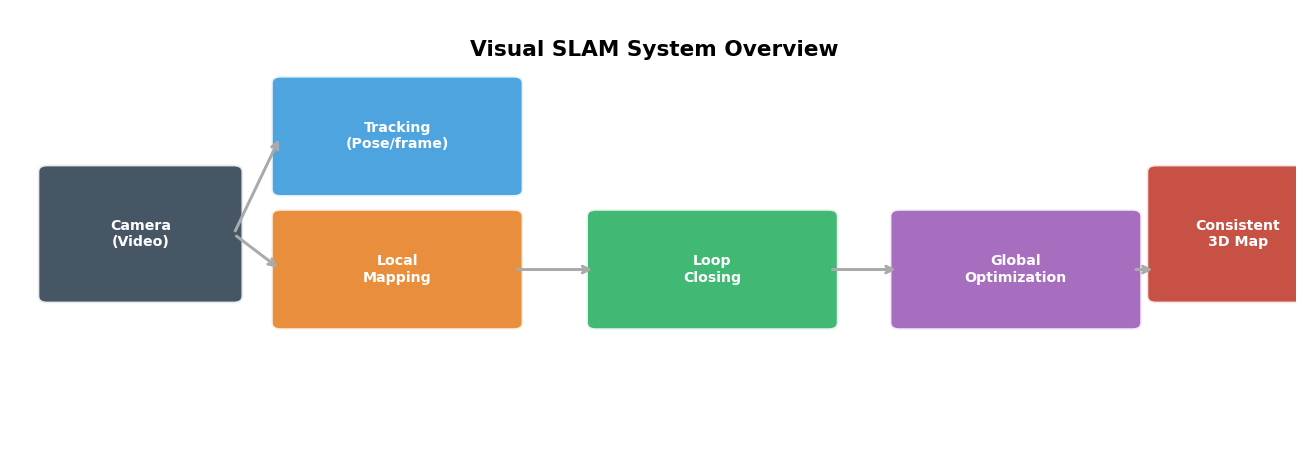
\includegraphics[width=0.85\textwidth]{images/slam_overview.png}
    \captionof{figure}{Sơ đồ hệ thống Visual SLAM. Camera cung cấp luồng ảnh liên tục. Module Tracking xác định pose theo thời gian thực. Module Local Mapping xây dựng bản đồ 3D cục bộ. Loop Closing phát hiện và sửa drift tích lũy.}
    \label{fig:slam_overview}
\end{center}

\subsubsection{Sai số Tích lũy và Loop Closing}
\label{subsubsec:drift_loop_closing}

Vấn đề cốt lõi của SLAM là \textbf{drift} (sai số tích lũy). Mỗi ước tính pose đều có một sai số nhỏ; khi robot di chuyển một đoạn dài, các sai số này cộng dồn, khiến bản đồ bị méo dần. Sau một hành trình dài, khi robot quay về điểm xuất phát, bản đồ có thể không khép kín—hai đầu của trajectory bị "lệch" nhau.

Loop Closing phát hiện: "Tôi đã từng đến đây rồi!" (bằng cách so sánh đặc trưng toàn cục như DBoW2, NetVLAD). Sau đó, Pose Graph Optimization phân bổ lại sai số:

\begin{center}
    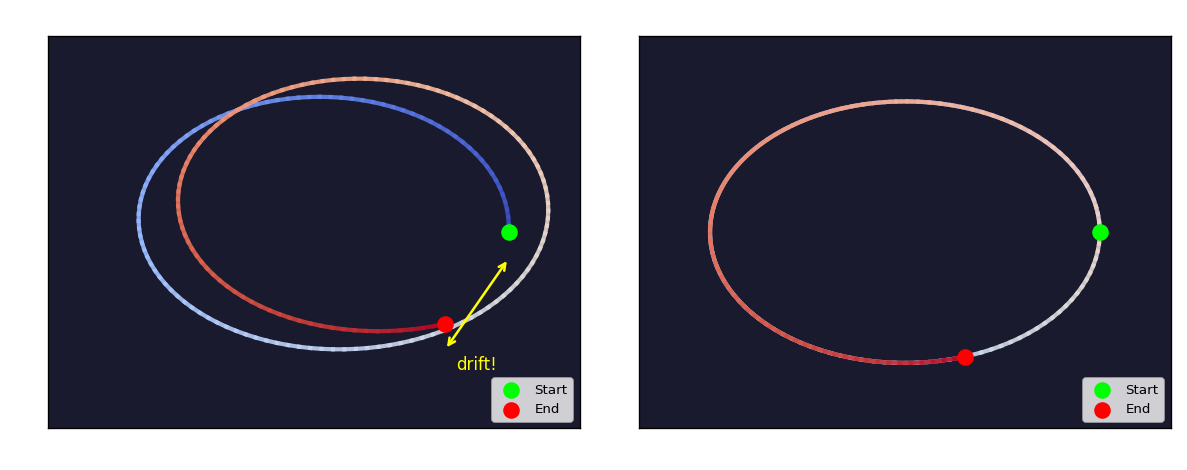
\includegraphics[width=0.8\textwidth]{images/loop_closing.png}
    \captionof{figure}{Minh họa tác dụng của Loop Closing. (Trái) Trajectory bị drift: khi quay về điểm xuất phát, hai đầu không khớp nhau. (Phải) Sau khi phát hiện vòng lặp và tối ưu hóa, trajectory được khép kín và bản đồ trở nên nhất quán.}
    \label{fig:loop_closing}
\end{center}

\subsection{SfM, SLAM và Tương lai: NeRF và Gaussian Splatting}
\label{subsec:sfm_to_nerf}

SfM và SLAM là các phương pháp biểu diễn cảnh 3D dưới dạng \textit{đám mây điểm (point cloud)} hoặc \textit{lưới tam giác (mesh)}—các biểu diễn rời rạc, tường minh. Trong Chương 8, chúng ta sẽ gặp một thế hệ phương pháp mới—\textbf{NeRF} và \textbf{Gaussian Splatting}—biểu diễn cảnh 3D \textit{ngầm định} bằng mạng nơ-ron hoặc Gaussian phân phối, cho chất lượng tái tạo và rendering đẹp hơn nhiều. Điều thú vị: cả NeRF lẫn Gaussian Splatting đều sử dụng \textbf{poses camera từ COLMAP} làm đầu vào—một lần nữa khẳng định tầm quan trọng nền tảng của hình học camera và SfM.

\section*{Tài liệu tham khảo}
\begin{itemize}
    \item[1] Schonberger, J.L.; Frahm, J.M. Structure-from-Motion Revisited. In \textit{CVPR}, 2016.
    \item[2] Campos, C. et al. ORB-SLAM3: An Accurate Open-Source Library for Visual, Visual–Inertial, and Multimap SLAM. \textit{IEEE Transactions on Robotics} \textbf{2021}.
    \item[3] Hartley, R.; Zisserman, A. \textit{Multiple View Geometry in Computer Vision}. Cambridge University Press, 2003.
\end{itemize}
